\chapter[ANÁLISIS]{ANÁLISIS DE RESULTADOS}
En este capítulo se presentan los resultados obtenidos en la implementación del chatbot utilizando
la plataforma Rasa OpenSource para responder preguntas frecuentes de estudiantes de la Facultad de
Ingeniería.  Además, se analizan los datos recopilados durante el entrenamiento del modelo, se
discuten las limitaciones, evaluara la efectividad del chatbot, asi como tambien posibles mejoras
en la implementación del chatbot.

\section{Configuraciones ulilizadas}
Dado el interés en que los resultados obtenidos sean replicables, en primer lugar, se explicarán
los componentes seleccionados para el entrenamiento y despliegue del modelo.
\begin{itemize}
	\item \textbf{WhitespaceTokenizer}: componente que divide el texto en palabras
	      individuales, utilizando espacios en blanco como delimitador.
	      \cite{Configuration_Documentation}
	\item \textbf{RegexFeaturizer}: componente que crea características basadas en expresiones
	      regulares. Esto puede ser útil para detectar patrones en el texto.
	      \cite{Configuration_Documentation}
	\item \textbf{LexicalSyntacticFeaturizer}: componente que combina características léxicas y
	      sintácticas para crear una mejor representación del texto. Utiliza etiquetas de
	      partes del discurso
	      y etiquetas de análisis de dependencia para crear características.
	      \cite{Configuration_Documentation}
	\item \textbf{CountVectorsFeaturizer}: componente que crea una representación dispersa de
	      bolsa de
	      palabras del texto. Puede ser utilizado para crear características para la
	      clasificación de
	      intenciones o la extracción de entidades. \cite{Configuration_Documentation}
	\item \textbf{DIETClassifier}: componente que combina una red neuronal recurrente con un
	      transformador para realizar la clasificación de intenciones y el reconocimiento de
	      entidades.
	      Utiliza múltiples fuentes de información, como incrustaciones de palabras,
	      incrustaciones de
	      caracteres y etiquetas de partes del discurso. \cite{Configuration_Documentation}
	\item \textbf{EntitySynonymMapper}: componente que mapea las entidades a su forma canónica.
	      Esto
	      puede ser útil para manejar variaciones en la forma en que se expresan las entidades
	      en el texto. \cite{Configuration_Documentation}
	\item \textbf{ResponseSelector}: componente que selecciona una respuesta basada en la
	      entrada del
	      usuario. Utiliza un enfoque basado en recuperación, donde coincide la entrada del
	      usuario con un
	      conjunto de respuestas predefinidas. Puede ser útil para manejar preguntas frecuentes
	      o
	      conversaciones informales.\cite{Configuration_Documentation}
	\item \textbf{FallbackClassifier}: componente que clasifica los mensajes como fallback si
	      no
	      coinciden con ninguna de las intenciones en el modelo. Puede ser útil para manejar
	      mensajes fuera
	      de contexto o solicitudes que el modelo no está entrenado para
	      manejar.\cite{Configuration_Documentation}
\end{itemize}
\section{Conjunto de Datos propio}

Inicialmente, se creó un conjunto de datos con las posibles preguntas frecuentes de los alumnos,
una vez que el Bot estuvo en funcionamiento e integrado a Telegram se recolectaron las preguntas
que realmente tienen los estudiantes de la FIUNA, estas fueron guardadas en una base de datos como
eventos, teniendo mucha información innecesaria para el conjunto de datos. Para un mejor manejo y
limpieza de los datos se utilizó Python con ayuda de la librería Pandas. Posteriormente se guardó
el dataframe creado en un archivo de Excel donde se analizaron y clasificaron un total de 1051
entradas en 141 intenciones distintas, De entre ellas, se identificaron las 15 intenciones más
recurrentes.

\begin{figure}[H]
	\centering
	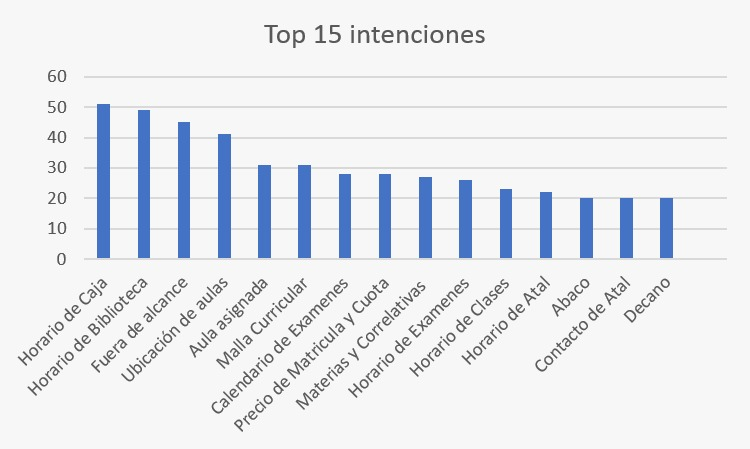
\includegraphics[width=\textwidth]{imagenes/cap5/Top15intents.jpeg}
	\caption{Top 15 Intenciones}
	\label{fig:Top15intents}
\end{figure}

\section{Validación de los datos e Historias}
Rasa cuenta con varias funciones para probar los diálogos, historias, gestor de diálogos y el
procesamiento de mensajes, de tal forma a encontrar errores o inconsistencias antes de realizar el
entrenamiento.

\subsection{Validación de datos}
El siguiente comando se encarga de verificar que no haya errores e inconsistencias en los datos y
configuraciones.

\begin{center}
	\framebox[10cm][c]{rasa data validate}
\end{center}

Es recomendable ejecutarlo antes de entrenar el modelo, ya que si se encuentra algún problema, el
entrenamiento también podría fallar.

\subsection{Evaluación del desempeño de la NLU}
Una práctica usual al ejecutar aprendizaje automático es dividir aleatoriamente el conjunto de
datos en uno de entrenamiento y otro de pruebas. El bot utiliza el primer conjunto para aprender
las características necesarias para realizar las predicciones adecuadas, y el segundo conjunto para
evaluar el modelo mediante datos que aún no hayan sido vistos antes.\\
Rasa nos permite dividir los datos mediante el comando:

\begin{center}
	\framebox[10cm][c]{rasa data split nlu}
\end{center}

Por defecto, Rasa separa los datos de entrenamiento/prueba en un 80/20, luego, para probar que tan
bien entrenado se encuentra el modelo utilizamos 'rasa test nlu' especificando cuales son los datos
de entrenamiento y prueba de la siguiente forma:\\

\begin{center}
	\framebox[10cm][c]{    --nlu train\_test\_split/test\_data.yml}
\end{center}

Rasa test proporciona herramientas que facilitan la detección y corrección de errores, incluye una
matriz de confusión, un archivo .json de reporte, un histograma de confianza y un archivo .json de
errores en caso de que existan.\\
La matriz de confusión es una herramienta fundamental que permite evaluar el rendimiento de un
modelo, permite identificar los falsos positivos y falsos negativos, nos muestra en su eje vertical
las etiquetas reales y en el eje horizontal las etiquetas predecidas, permitiendo identificar si
existen errores de clasificación.\\
Además, el script de rasa test guarda estos errores de clasificación en un archivo .json lo que
facilita el depurado y corrección de errores para mejorar la calidad de la clasificación.\\
El Histograma nos permite visualizar las predicciones del modelo y la confianza que ha sido
otorgada a cada intención o entidad.\\
Las predicciones correctas se encuentran en la parte izquierda del gráfico y son representadas en
color azul, mientras que las incorrectas se encuentran a la derecha y son de color rojo.\\
La ubicación de cada predicción en el eje horizontal del histograma representa el número de
muestras, y en el eje vertical la confianza con la que el modelo ha realizado su
predicción. \cite{interpretacion_graficos}

\subsection{Clasificador de Intenciones}

\begin{figure}[H]
	\centering
	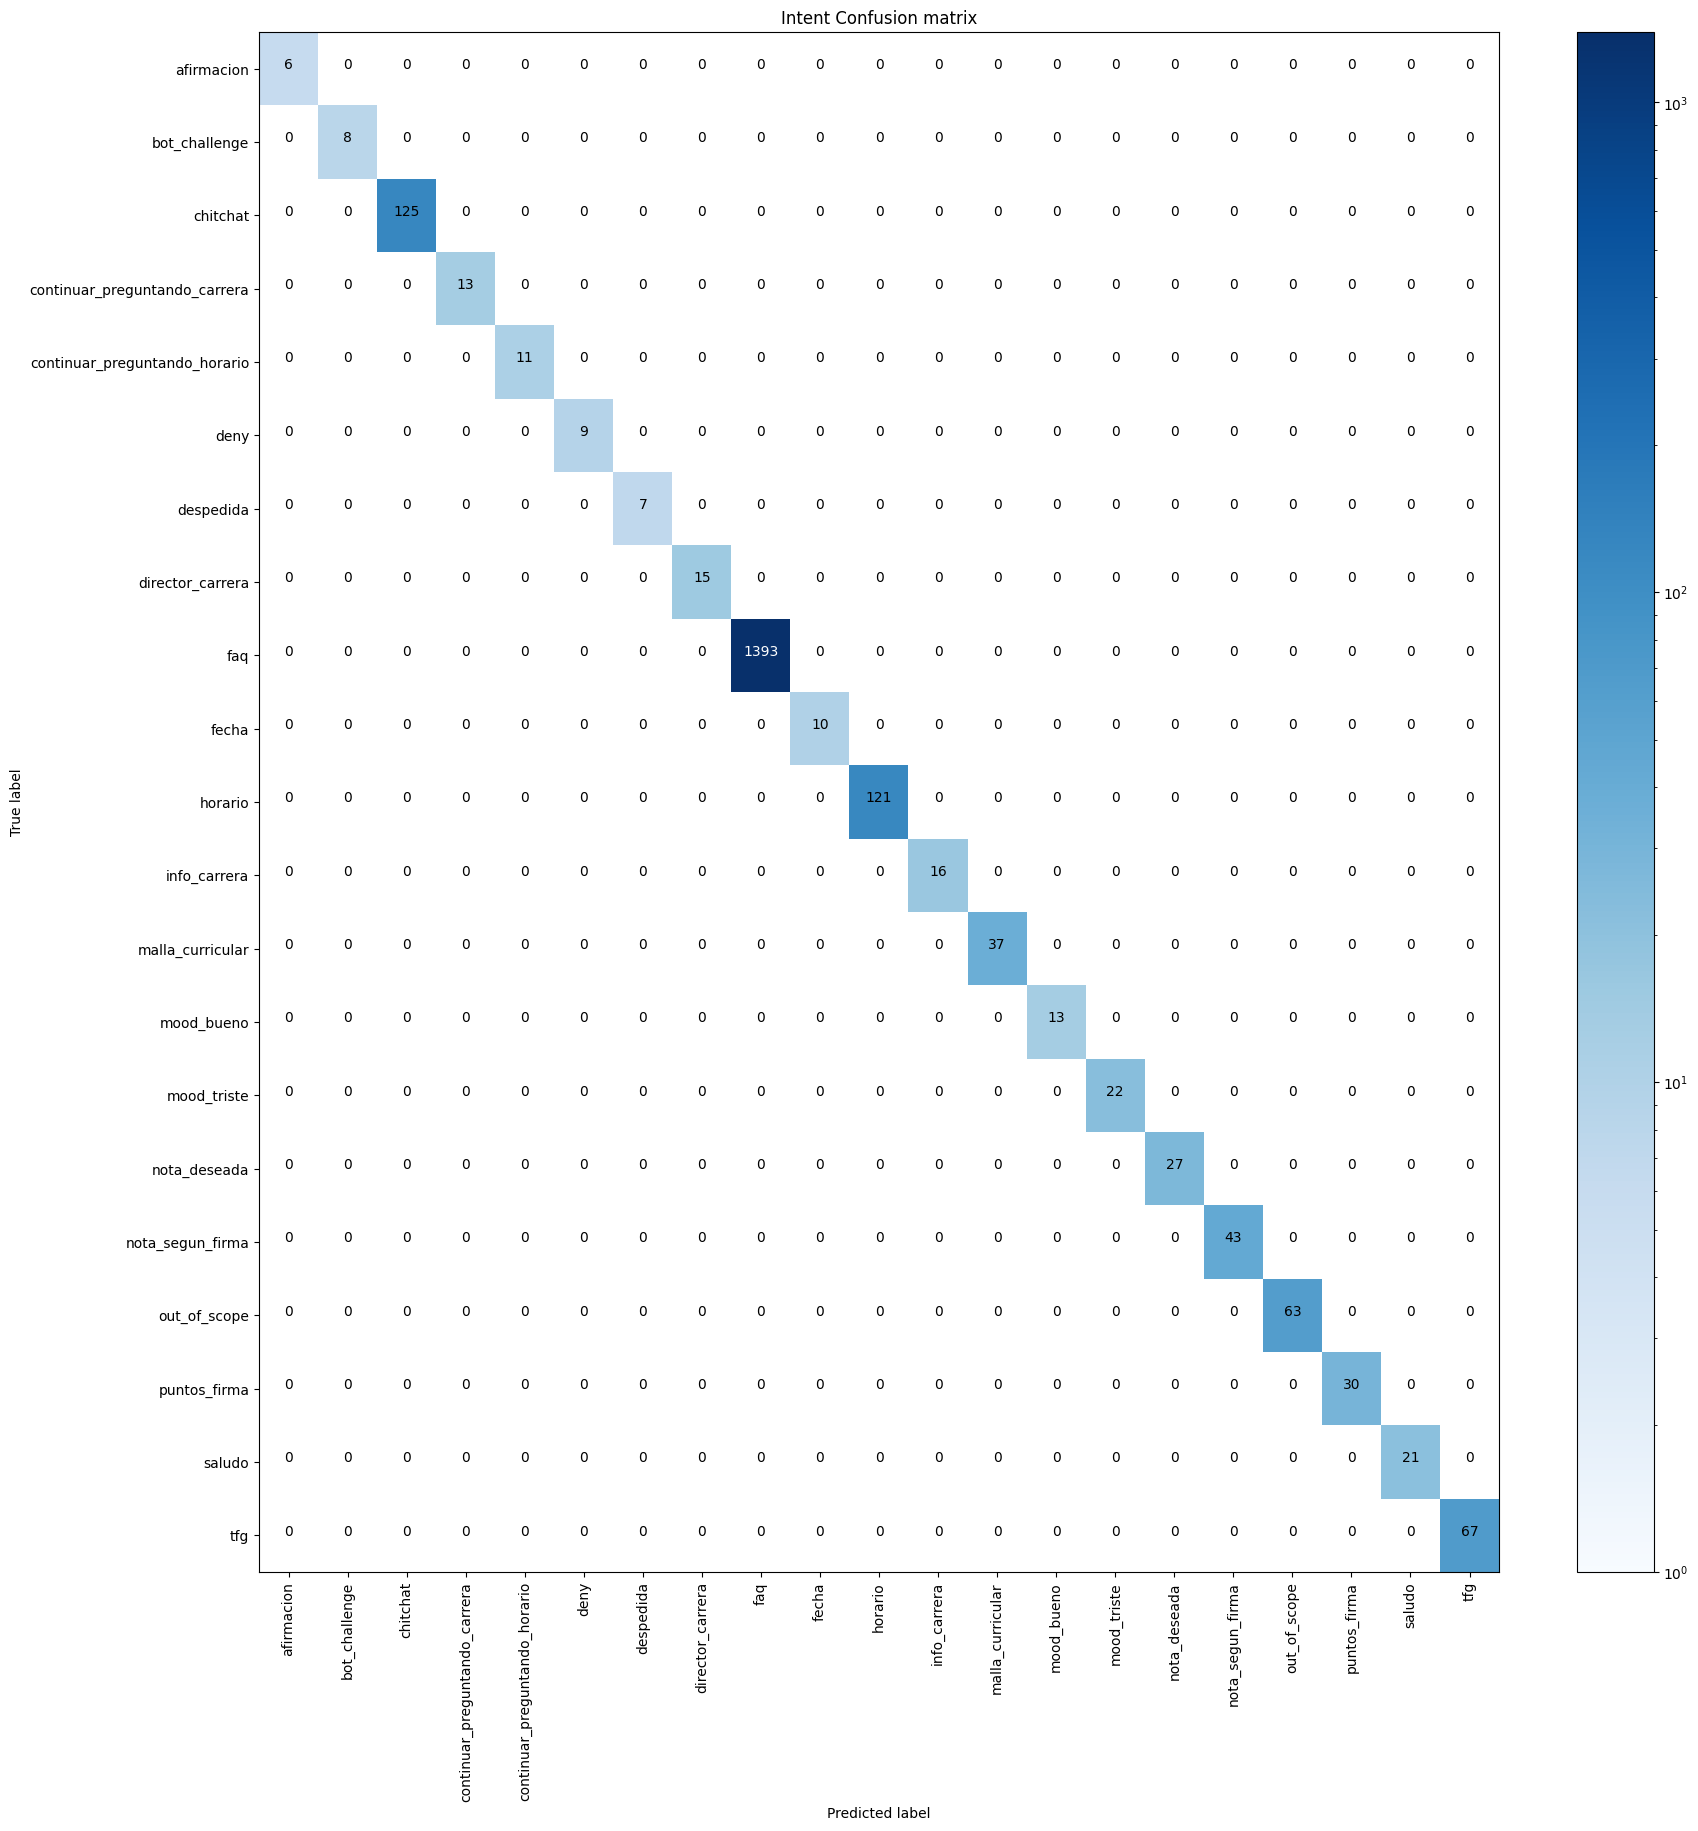
\includegraphics[width=\textwidth]{imagenes/cap5/intent_confusion_matrix.png}
	\caption{Matriz de Confusión de Intenciones}
	\label{fig:intent_matriz}
\end{figure}

\begin{figure}[H]
	\centering
	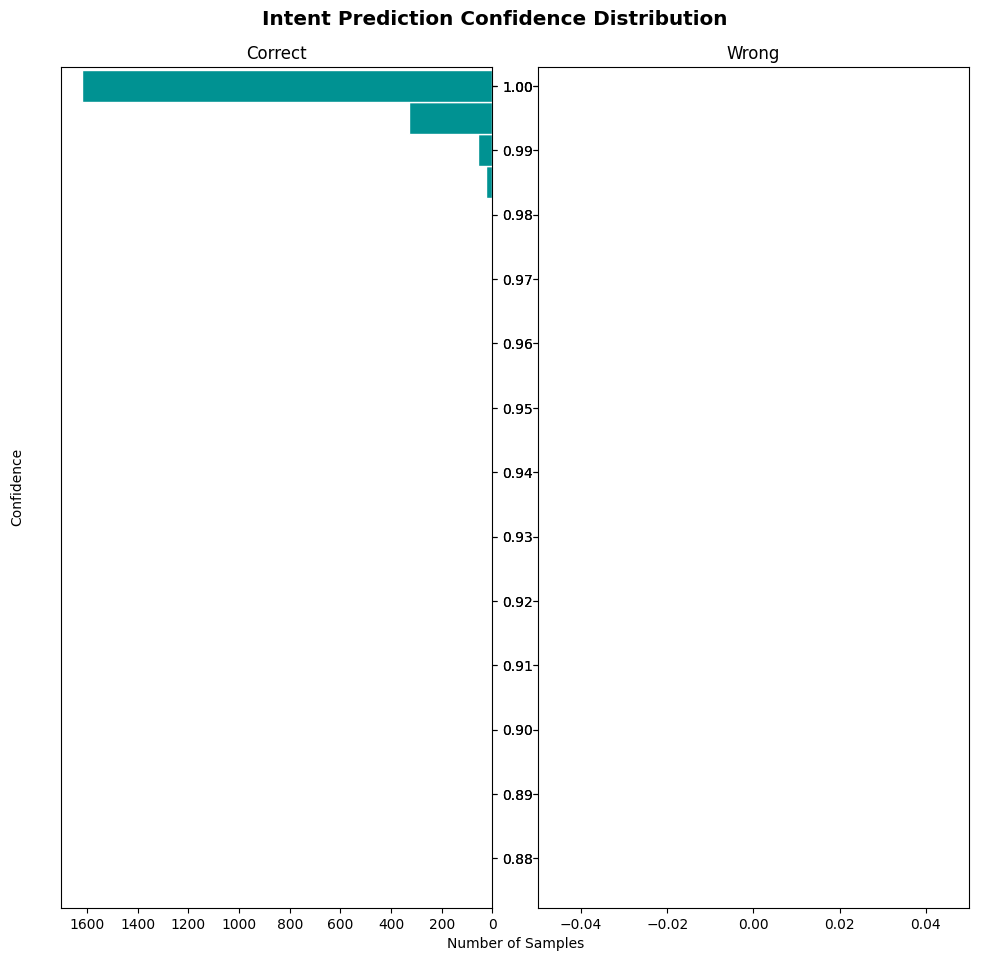
\includegraphics[width=\textwidth]{imagenes/cap5/intent_histogram.png}
	\caption{Histograma de confianza en la clasificación de Intenciones}
	\label{fig:intent_histograma}
\end{figure}

Al analizar la matriz de confusión \ref{fig:intent_matriz} y el histograma
\ref{fig:intent_histograma} podemos verificar que todas las intenciones fueron clasificadas
correctamente con una confianza superior a 0.98, indicando que el modelo es bastante efectivo en su
tarea de clasificación.
\subsection{Extracción de entidades}
Al ver los gráficos del extractor, tanto en la matriz de confusión de entidades
\ref{fig:entity_matriz} como en el histograma \ref{fig:entity_histograma} se encuentra que el
modelo se confunde con dos entidades, revisando el reporte de errores se encuentra que los
extractores DIETClassifier y EntitySynonymMapper reconocen las entidades por separado, esto genera
el error pero no afecta al rendimiento del modelo o a la correcta selección de una respuesta.

\begin{figure}[H]
	\centering
	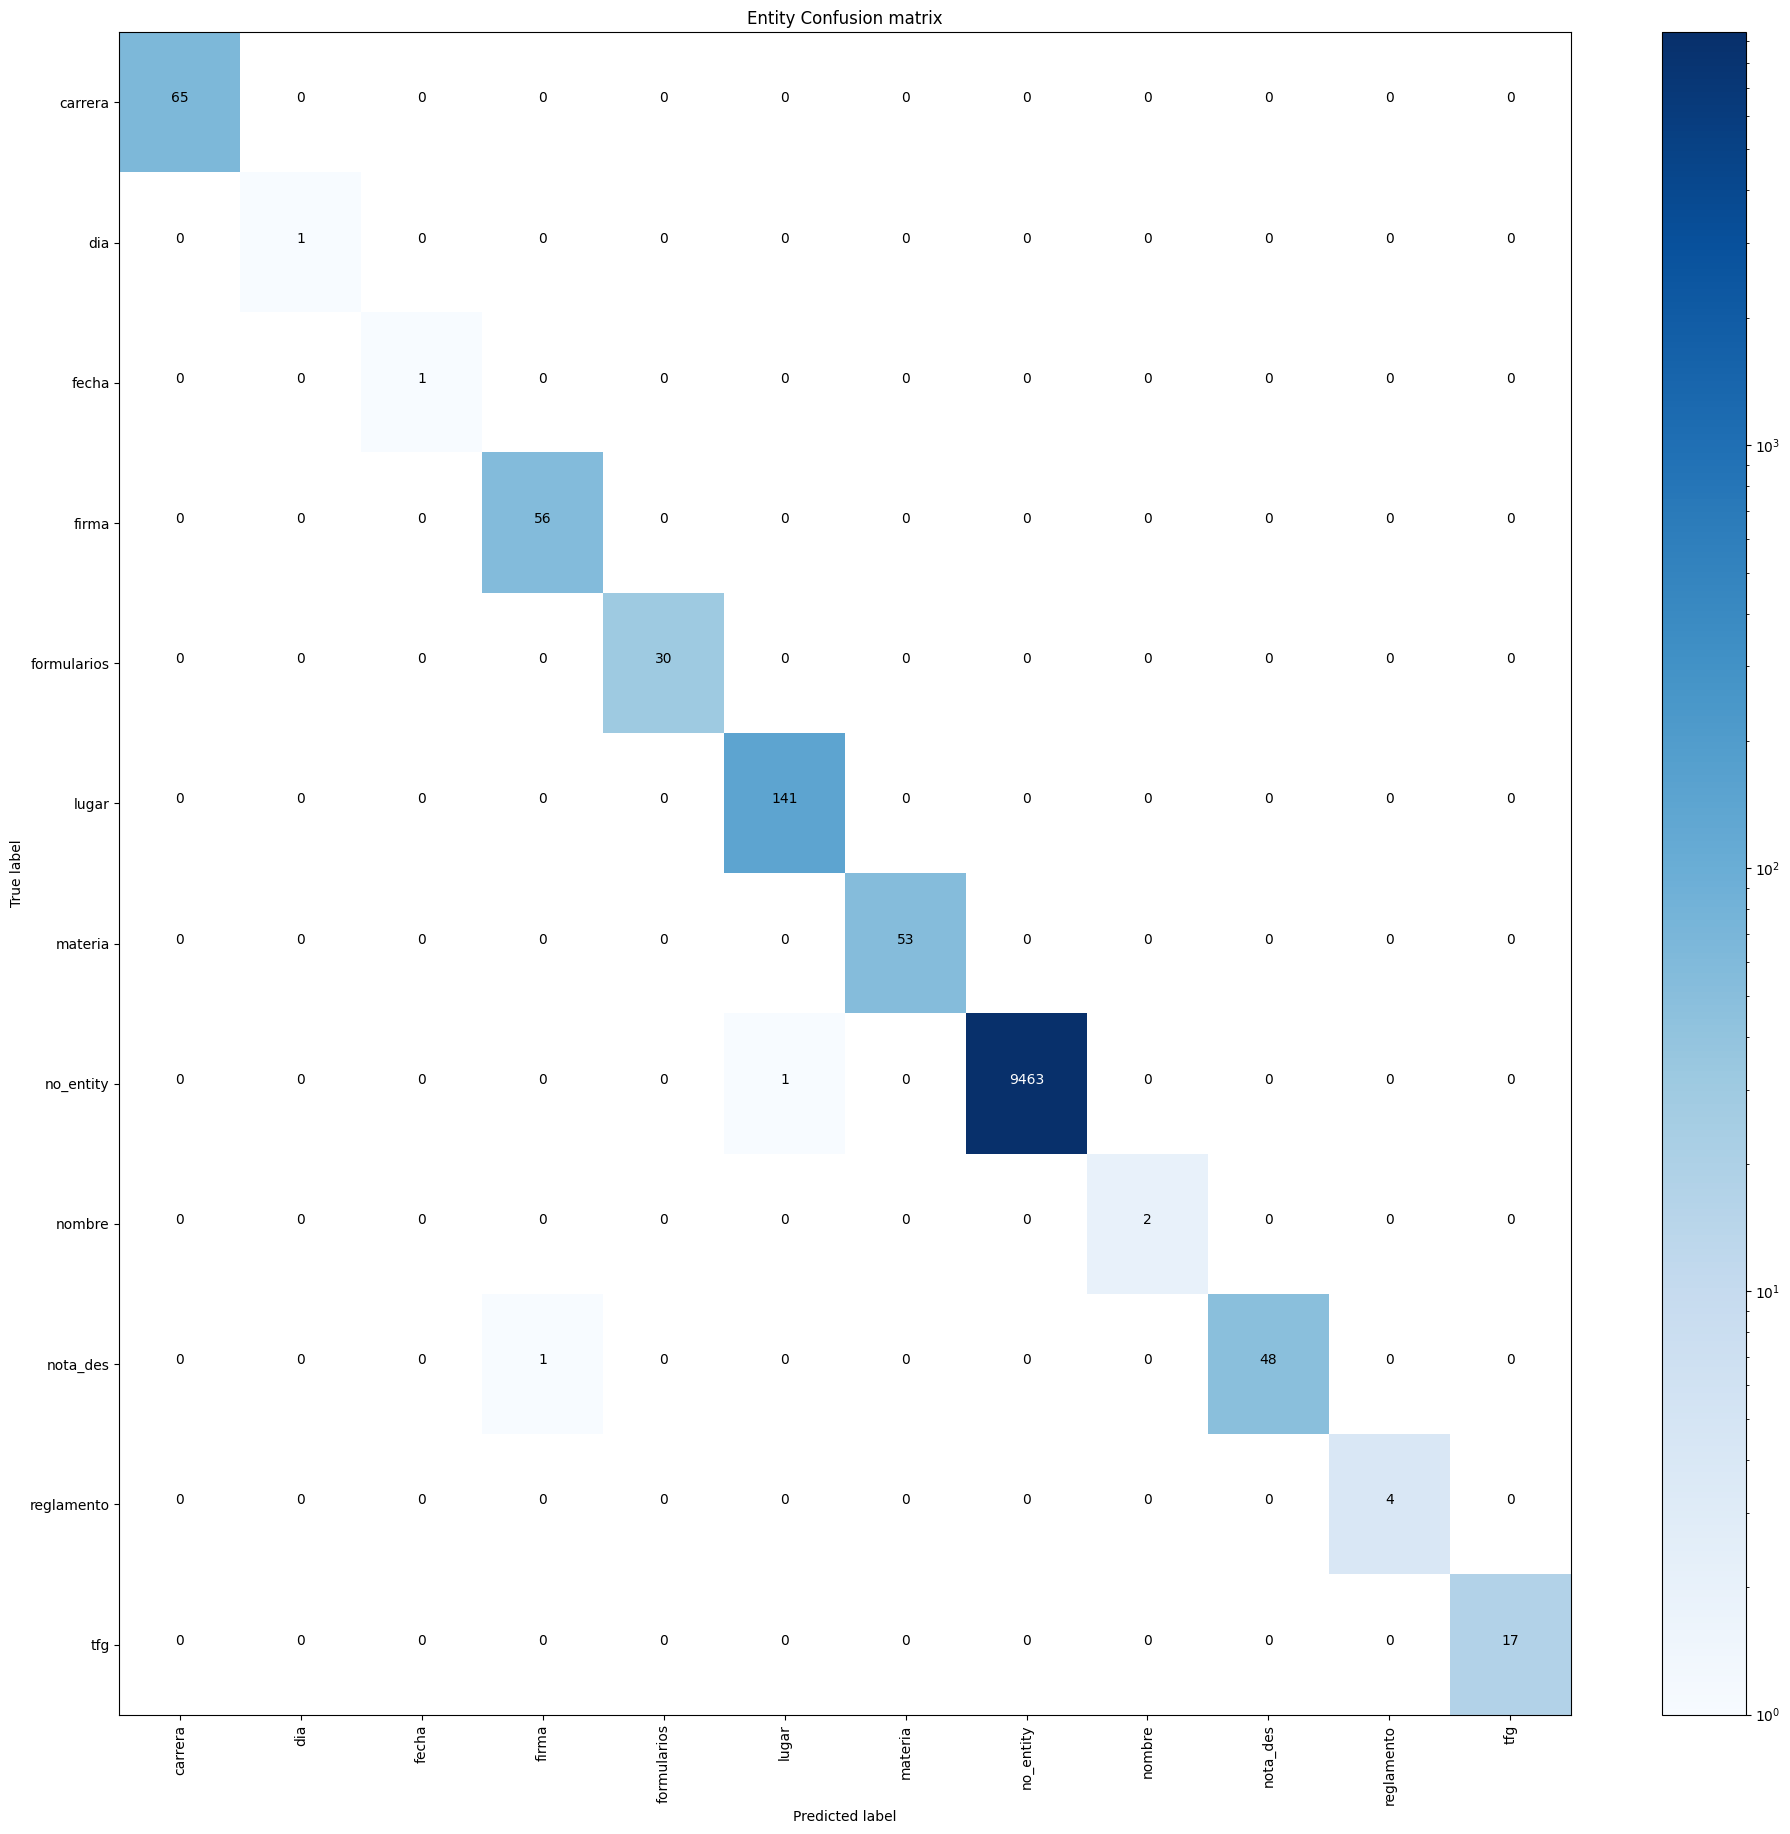
\includegraphics[width=\textwidth]{imagenes/cap5/DIETClassifier_confusion_matrix.png}
	\caption{Matriz de Confusión del extractor de entidades}
	\label{fig:entity_matriz}
\end{figure}

\begin{figure}[H]
	\centering
	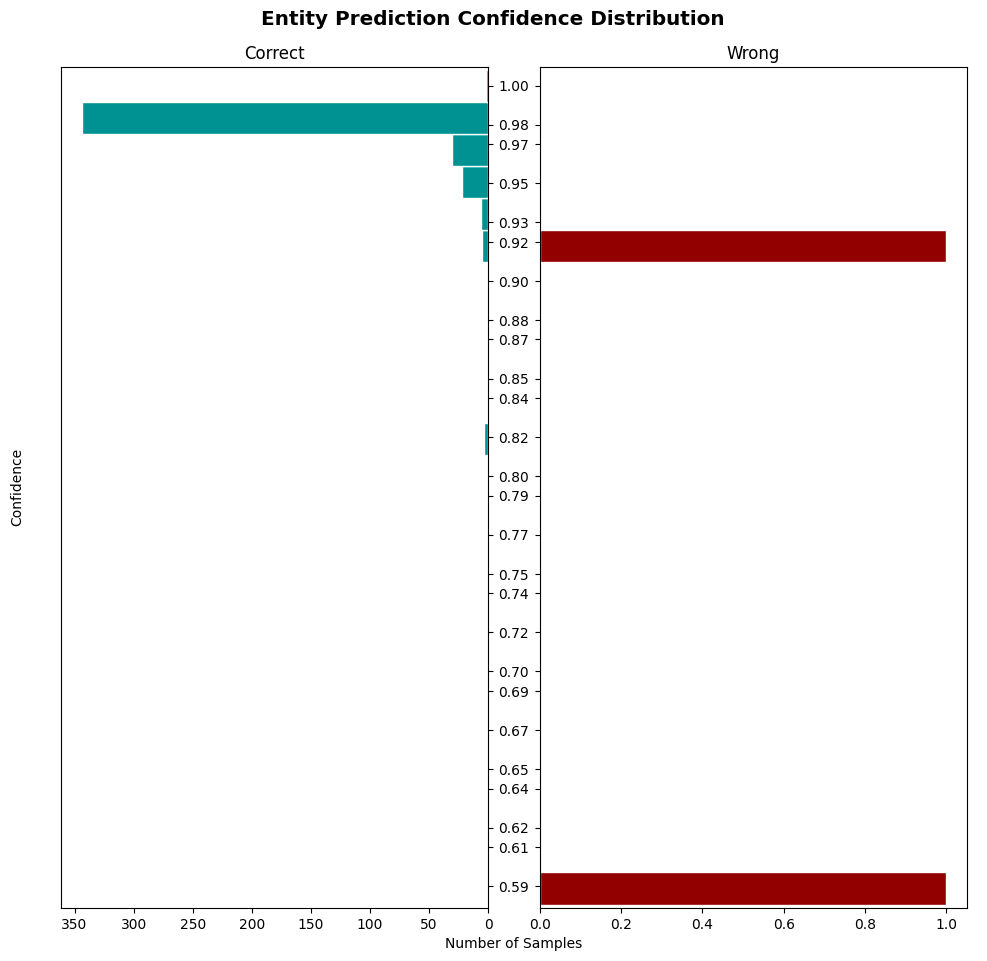
\includegraphics[width=\textwidth]{imagenes/cap5/DIETClassifier_histogram.png}
	\caption{Histograma de confianza del extractor de entidades}
	\label{fig:entity_histograma}
\end{figure}

\subsection{Selección de Respuestas}
Podemos observar en el histograma \ref{fig:response_histograma} de la selección de respuestas que
no se predijo erróneamente ninguna respuesta, la matriz de confusión en este caso no es de mucha
utilidad ya que son bastantes respuestas y complica la visibilidad de las etiquetas, en caso de que
existiese un error podremos encontrarlo en el reporte .json.

\begin{figure}[H]
	\centering
	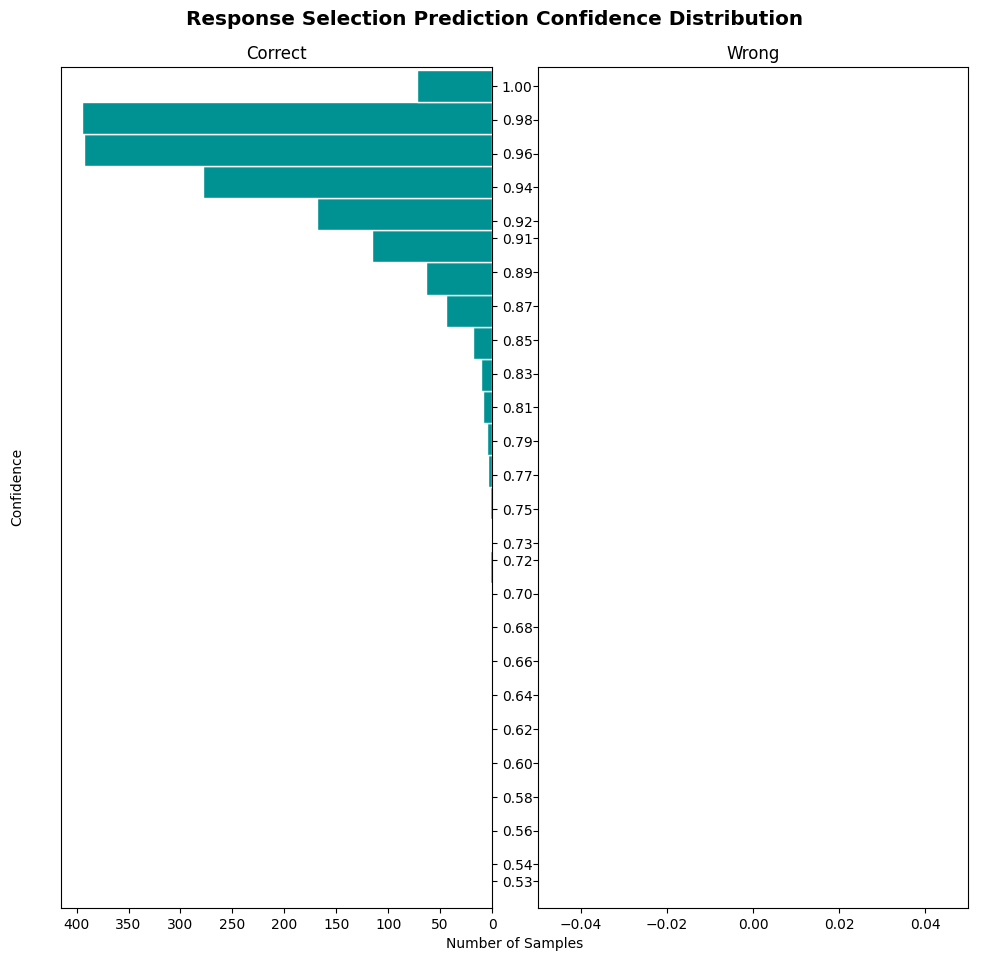
\includegraphics[width=\textwidth]{imagenes/cap5/response_selection_histogram.png}
	\caption{Histograma de confianza del seleccionador de respuestas}
	\label{fig:response_histograma}
\end{figure}

\section{Posibles Mejoras}
\begin{itemize}
	\item Integrar a sistemas existentes de la Facultad de Ingeniería.
	\item Se puede agregar respuestas de la chatbots públicos como	ChatGPT \cite{api_chatgpt}
	      para preguntas
	      fuera del
	      contexto de la Facultad de Ingeniería.
\end{itemize}
\chapter[Glosario]{Glosario}
\begin{itemize}
	\item \textbf{Acciones:} son funciones que se utilizan para realizar tareas en una conversación, pueden ser simples como respuestas genéricas o mas personalizadas con un código Python.
	\item \textbf{Aprendizaje Automático o de Máquina (Machine Learning):} es un subcampo de la inteligencia artificial que se enfoca en el desarrollo de algoritmos y modelos estadísticos que permiten a los sistemas informáticos aprender automáticamente de los datos, sin ser programados explícitamente para ello 
	\item \textbf{Aprendizaje Profundo (Deep Learning):} es una técnica de aprendizaje automático basada en redes neuronales artificiales de múltiples capas, que se utilizan para aprender patrones complejos y realizar tareas avanzadas como el reconocimiento de imágenes, voz y lenguaje natural.
	\item \textbf{Caracterizadores:} son herramientas de procesamiento de lenguaje natural que convierten texto en vectores numéricos utilizados para entrenar modelos de aprendizaje automático
	\item \textbf{Chatbot:} programas que imitan la conversación humana, capaces de interactuar con las personas y de responder adecuadamente a sus preguntas.
	\item \textbf{Conjunto de datos (Dataset):} es un conjunto de observaciones o ejemplos utilizados para entrenar modelos de aprendizaje automático
	\item \textbf{Contenedor:} forma de empaquetar y distribuir aplicaciones y sus dependencias junto con su configuración y recursos necesarios para su ejecución en diferentes entornos.
	\item \textbf{Docker:} plataforma de contenedores de software que permite empaquetar, distribuir y ejecutar aplicaciones y sus dependencias en entornos aislados.
	\item \textbf{Entidades:} representa un objeto o un concepto en una parte del texto, por ejemplo lugar o carrera.
	\item \textbf{Entorno Virtual:} herramienta que permite crear y gestionar un ambiente de trabajo aislado en un sistema operativo, con sus propias dependencias y configuraciones
	\item \textbf{Formularios:} son una manera de recopilar información necesaria para llevar a cabo una acción específica.
	\item \textbf{Intenciones:} en un mensaje del usuario, la intención es lo que se pretende transmitir o lograr
	\item \textbf{NLU:} se ocupa de analizar y comprender el lenguaje humano en un formato estructurado.
	\item \textbf{Procesamiento de Lenguaje Natural (NLP):} Campo de ciencias de Computación y la Lingüística que trata con métodos para analizar, modelar y entender el lenguaje humano.
	\item \textbf{Rasa Core:} forma parte de la librería Rasa, es el motor de diálogo que decide qué hacer a continuación en una conversación en función del contexto.
	\item \textbf{Rasa NLU:} es la parte de Rasa que realiza la comprensión del lenguaje natural (NLU), incluida la clasificación de intenciones y la extracción de entidades.
	\item \textbf{Reglas:} indica un comportamiento que se debe seguir en la conversación, donde una condición específica siempre predice una próxima acción específica.
	\item \textbf{Slots:} variables utilizadas para guardar información a lo largo de la conversación.
	\item \textbf{Tesauro:} vocabulario controlado y estructurado que se utiliza para indexar y recuperar información por medio de conceptos relacionados.
	\item \textbf{Tokenizadores:} herramienta utilizada en el procesamiento de lenguaje natural que divide el texto en unidades básicas de procesamiento de texto.
	\item \textbf{Transformadores:} tipo de arquitectura de redes neuronales utilizada en el procesamiento de lenguaje natural.
\end{itemize}
